\section{Introduction}

% ------------------------------------------------------------------------------
\begin{frame}{Can a decision model give LLM quality at IDE speed?}
  \centering
  \begin{tikzpicture}[x=1mm, y=1mm]
    % latency budgets of the three places where leak checks run
    \foreach \x/\w/\name/\t in {0/34/IDE/< 0.1\,s, 36/34/pre-commit/< 1\,s, 72/34/CI/< 10\,s}{
      \node[box, minimum width=\w mm, minimum height=10mm] at (\x+\w/2, 0) {\textbf{\name}\\{\small \t}};
    }
    \draw[arr] (0,-8) -- node[lbl, below] {analysis must be fast} (106,-8);
    % generative vs decision model
    \node[warn, minimum width=44mm, minimum height=15mm, align=center] (gen) at (20,-27)
      {\textbf{Generative LLM}\\{\small writes an answer}\\{\small accurate, but slow and paid}};
    \node[data, minimum width=44mm, minimum height=15mm, align=center] (dec) at (86,-27)
      {\textbf{Decision model}\\{\small outputs one score}\\{\small no text generation}};
    \draw[arr, dashed] (gen.east) -- node[lbl, above] {same quality?} (dec.west);
  \end{tikzpicture}
  \vspace{6pt}

  \textbf{Question:} near-LLM quality at decision-model speed?\\[2pt]
  {\small Task: C/C++ memory leaks (CWE-401) in Juliet units}
\end{frame}

% ------------------------------------------------------------------------------
\begin{frame}{On original Juliet, a one-line rule beats every static analyzer}
  \begin{columns}[c]
    \begin{column}{0.57\textwidth}
      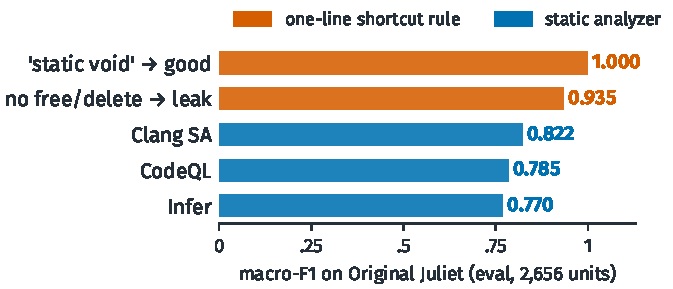
\includegraphics[width=\linewidth]{figures/hook_original.pdf}
    \end{column}
    \begin{column}{0.41\textwidth}
      \begin{itemize}
        \item Good: \code{static} helpers
        \item Bad: no \code{free}
        \item Templates reveal labels
      \end{itemize}
      \vspace{6pt}
      \alert{Scores are untrustworthy.}\\
      Rebuild the benchmark first.
    \end{column}
  \end{columns}
  \vfill
  {\scriptsize Template shortcuts: Germano et al.\ (ICAART'25); Risse \& B\"ohme (USENIX Sec'24).\par}
\end{frame}
